\documentclass[UTF8,a4paper,10pt]{ctexart}
\usepackage[left=2.50cm, right=2.50cm, top=2.50cm, bottom=2.50cm]{geometry}
%页边距
\CTEXsetup[format={\Large\bfseries}]{section} %设置章标题居左

%%%%%%%%%%%%%%%%%%%%%%%
% -- text font --
% compile using Xelatex
%%%%%%%%%%%%%%%%%%%%%%%
% -- 中文字体 --
%\setmainfont{Microsoft YaHei}  % 微软雅黑
%\setmainfont{YouYuan}  % 幼圆    
%\setmainfont{NSimSun}  % 新宋体
%\setmainfont{KaiTi}    % 楷体
%\setmainfont{SimSun}   % 宋体
%\setmainfont{SimHei}   % 黑体
% -- 英文字体 --
%\usepackage{times}
%\usepackage{mathpazo}
%\usepackage{fourier}
%\usepackage{charter}
%%
%\usepackage{helvet}
\usepackage{amsmath, amsfonts, amssymb} % math equations, symbols
\usepackage[english]{babel}
\usepackage{color}	% color content
\usepackage{graphicx}	% import figures
\usepackage{url}	% hyperlinks
\usepackage{bm} 	% bold type for equations
\usepackage{multirow}
\usepackage{booktabs}
\usepackage{epstopdf}
\usepackage{epsfig}
\usepackage{algorithm}
\usepackage{algorithmic}
\usepackage{listings}
\usepackage{xcolor}
\usepackage{booktabs}
\usepackage{zhnumber}
\usepackage{longtable}
\usepackage{subfigure}
\usepackage{float}
\renewcommand\thesection{\zhnum{section}}
\renewcommand \thesubsection {\arabic{section}}
\renewcommand{\algorithmicrequire}{ \textbf{Input:}}
% use Input in the format of Algorithm  
\renewcommand{\algorithmicensure}{ \textbf{Initialize:}}
% use Initialize in the format of Algorithm  
\renewcommand{\algorithmicreturn}{ \textbf{Output:}}
% use Output in the format of Algorithm  
%%%%%%%%%%%%%%%%%%
\usepackage{listings}
\usepackage{color}
\definecolor{dkgreen}{rgb}{0,0.6,0}
\definecolor{gray}{rgb}{0.5,0.5,0.5}
\definecolor{mauve}{rgb}{0.58,0,0.82}
\lstset{frame=tb,
  language=Python,
  aboveskip=3mm,
  belowskip=3mm,
  showstringspaces=false,
  columns=flexible,
  basicstyle={\small\ttfamily},
  numbers=left,%设置行号位置none不显示行号
  %numberstyle=\tiny\courier, %设置行号大小
  numberstyle=\tiny\color{gray},
  keywordstyle=\color{blue},
  commentstyle=\color{dkgreen},
  stringstyle=\color{mauve},
  breaklines=true,
  breakatwhitespace=true,
  escapeinside=``,%逃逸字符(1左面的键),用于显示中文例如在代码中`中文...`
  tabsize=4,
  extendedchars=false %解决代码跨页时,章节标题,页眉等汉字不显示的问题
}

%%%%%%%%%%%%%%%%%%%%%%%%%%%%
\usepackage{fancyhdr} %设置页眉、页脚
\pagestyle{fancy}
\lhead{}
\chead{}
%\rhead{\includegraphics[width=1.2cm]{fig/ZJU_BLUE.eps}}
\lfoot{}
\cfoot{}
\rfoot{}
\fancyfoot[RE,RO]{~\thepage~}

\fancyhead[RE,RO]{计算物理导论 \quad 2022春季学期 \quad 作业1  \quad 何翼成}

%%%%%%%%%%%%%%%%%%%%%%%
%  设置水印
%%%%%%%%%%%%%%%%%%%%%%%
%\usepackage{draftwatermark}         % 所有页加水印
%\usepackage[firstpage]{draftwatermark} % 只有第一页加水印
% \SetWatermarkText{Water-Mark}           % 设置水印内容
% \SetWatermarkText{\includegraphics{fig/ZJDX-WaterMark.eps}}         % 设置水印logo
% \SetWatermarkLightness{0.9}             % 设置水印透明度 0-1
% \SetWatermarkScale{1}                   % 设置水印大小 0-1    

\usepackage{hyperref} %bookmarks
\hypersetup{colorlinks, bookmarks, unicode} %unicode

\title{\textbf{0307计算物理导论作业}}
\author{ 何翼成 \thanks{学号:520072910043; \newline
    邮箱地址:heyicheng@sjtu. edu. cn} }
\date{\today}

\begin{document}
\maketitle

%\begin{abstract}
%这是一篇中文小论文。这个部分用来写摘要。摘要的章标题默认是英文,还没找到改成中文的方法:(
%\end{abstract}

\section{题目一}

%\section*{单摆的非线性振动}
\subsubsection{代码展示}

%代码展示的源代码
~\\
\lstset{language=matlab}
\begin{lstlisting}
  %%用辛普森公式求下面积分,结果精确到10^(-8)
  clear;clc;
  xspan=[0,1];
  x_0=xspan(1);x_2n=xspan(end);
  l=x_2n-x_0;
  y_0=dI(x_0);y_2n=dI(x_2n);
  error=10^(-8);
  maxn=10000;
  ints_series=zeros(1,maxn);
  for n=1:maxn
      s1=0;s2=0;
      for i=1:n
          s1=s1+dI((2*i-1)*l/(2*n)+x_0);
          s2=s2+dI((2*i)*l/(2*n)+x_0);
      end
      ints=l*(y_0-y_2n+4*s1+2*s2)/(6*n);
      ints_series(n)=ints;
      if n>1&&abs(ints_series(n)-ints_series(n-1))<error
          steps=n;
          s=ints;
          break
      end
  end
  format long
  fprintf("数值积分结果为"+num2str(s,9)+",其中辛普森法划分区间数为"+2*n)
  function dI=dI(x)
        dI=4./(1+x^2);
end
\end{lstlisting}
%代码展示的源代码
%~\\
%\lstset{language=python}
%\begin{lstlisting}
%\end{lstlisting}
\subsubsection{代码运行结果}
数值积分结果为3.14159265,其中辛普森法划分区间数为14。\newline

\section{题目二}
\subsubsection{代码展示}
~\\
\lstset{language=matlab}
\begin{lstlisting}
  %%
  %数值求解sinx/x不定积分
  clear;clc;
  f=@(x)sin(x)/x;
  error=10^(-8);
  maxn=100000;
  maxi=100;
  s=0;
  s_series=zeros(1,maxi);
  for i=1:maxi
       xspan=[2^(-i),2^i];
       s=simpson(xspan,f,maxn);
       s_series(i)=s;
       if i>1&&abs(s_series(i)-s_series(i-1))<10^(-8)
          break
       end
  end
  [delta_min,idelta_min]=min(abs(s_series-pi/2));
  fprintf("数值积分结果为"+num2str(s_series(idelta_min),9)+",
  其中积分区间为["+2^(-idelta_min)+","+2^(idelta_min)+"]")
  function dI=dI(x)
        dI=4./(1+x^2);
end
function s=simpson(xspan,f,maxn)
x_0=xspan(1);x_2n=xspan(end);
l=x_2n-x_0;
y_0=f(x_0);y_2n=f(x_2n);
s1=0;s2=0;
for i=1:maxn
     s1=s1+f((2*i-1)*l/(2*maxn)+x_0);
     s2=s2+f((2*i)*l/(2*maxn)+x_0);
end
s=l*(y_0-y_2n+4*s1+2*s2)/(6*maxn);
end
\end{lstlisting}


\subsubsection{代码运行结果}
数值积分结果为1.57079638,其中积分区间为[3.8147e-06,262144]。\newline

\section{题目三}
\subsection{第一类边界条件}
\subsubsection{代码展示}
~\\
\lstset{language=matlab}
\begin{lstlisting}
  clear;clc;
  x=-1:0.1:1;
  f=@(x)1./(1+x.^2);
  y=f(x);
  format short
  y0=y(1);          %  S'(x0)=f'(x0)=y0   
  yn=y(end);          %  S'(xn)=f'(xn)=yn
  x0=x;
  s=threesimple1(x,y,x0,y0,yn)
  plot(x0,s)        %绘制第一边界条件插值函数图像
  hold on
  grid on
  plot(x,y,'o')
  xlabel('自变量 X'), ylabel('因变量 Y')
  title('插值点与三次样条函数') 
  legend('三次样条插值点坐标','插值点')
  function [D,h,A,g,M]=three1(X,Y,y0,yn)
  %        自然边界条件的三次样条函数(第一种边界条件)
  %        此函数为M值求值函数
  %        D,h,A,g,M输出量分别为系数矩阵D,插值宽度h,差商表A,g值,M值 
           n=length(X); 
           A=zeros(n,n);A(:,1)=Y';D=zeros(n,n);g=zeros(n,1);
           for  j=2:n
              for i=j:n
                  A(i,j)=(A(i,j-1)- A(i-1,j-1))/(X(i)-X(i-j+1));
              end
           end
           
           for i=1:n-1
               h(i)=X(i+1)-X(i);
           end
           for i=1:n
               D(i,i)=2; 
               D(1,2)=1;
               D(n,n-1)=1;
               if (i==1)
                   g(i,1)=6/h(i)*(A(2,2)-y0); 
               elseif (i==n) 
                       g(i,1)=6/h(i-1)*(yn-A(i,2));
               else 
                   g(i,1)=(6/(h(i-1)+h(i)))*(A(i+1,2)-A(i,2));
               end
             
           end  
           for i=1:n-2
               u(i)=h(i)/(h(i)+h(i+1));
               n(i)=1-u(i);  
               D(i+1,i+2)=n(i);
               D(i+1,i)=u(i);             %改到这里
           end
           M=D\g;
           %M=[0;M;0];         
  end
  function s=threesimple1(X,Y,x,y0,yn)
  %        三次样条插值函数第一类型代码 
  %        s函数表示三次样条插值函数插值点对应的函数值
  %        根据三次样条参数函数求出的D,h,A,g,M
  %        x表示求解插值点函数点,X为已知插值点        
           [D,h,A,g,M]=three1(X,Y,y0,yn)
           n=length(X); m=length(x);    
           for t=1:m
              for i=1:n-1
                 if (x(t)<=X(i+1))&&(x(t)>=X(i))
                    p1=M(i,1)*(X(i+1)-x(t))^3/(6*h(i));
                    p2=M(i+1,1)*(x(t)-X(i))^3/(6*h(i));
                    p3=(A(i,1)-M(i,1)/6*(h(i))^2)*(X(i+1)-x(t))/h(i);
                    p4=(A(i+1,1)-M(i+1,1)/6*(h(i))^2)*(x(t)-X(i))/h(i);
                    s(t)=p1+p2+p3+p4; 
                    break;
                 else
                     s(t)=0; 
                 end
              end
           end
  end
  function [D,h,A,g,M]=three2(X,Y,y0,yn)
  %        第二边界条件的三次样条函数(包含自然边界条件)
  %        y0,yn表示的是S''(x0)=f''(x0)=y0,S''(xn)=f''(xn)=yn,自然边界即条件值为0 
  %        此函数为M值求值函数
  %        D,h,A,g,M输出量分别为系数矩阵D,插值宽度h,差商表A,g值,M值 
           n=length(X); 
           A=zeros(n,n);A(:,1)=Y';D=zeros(n-2,n-2);g=zeros(n-2,1);
           for  j=2:n
              for i=j:n
                  A(i,j)=(A(i,j-1)- A(i-1,j-1))/(X(i)-X(i-j+1));
              end
           end
           
           for i=1:n-1
               h(i)=X(i+1)-X(i);
           end        
           for i=1:n-2
               D(i,i)=2;
               if (i==1)
                   g(i,1)=(6/(h(i+1)+h(i)))*(A(i+2,2)-A(i+1,2))-h(i)/(h(i)+h(i+1))*y0;
               elseif (i==(n-2))
                   g(i,1)=(6/(h(i+1)+h(i)))*(A(i+2,2)-A(i+1,2))-(1-h(i)/(h(i)+h(i+1)))*yn;
               else
                   g(i,1)=(6/(h(i+1)+h(i)))*(A(i+2,2)-A(i+1,2));
               end             
           end
           for i=2:n-2
               u(i)=h(i)/(h(i)+h(i+1));
               n(i-1)=h(i)/(h(i-1)+h(i));
               D(i-1,i)=n(i-1);
               D(i,i-1)=u(i);             
           end
           M=D\g;
           M=[y0;M;yn];         
  end
  function s=threesimple2(X,Y,x,y0,yn)
  %        第二边界条件函数 
  %        s函数表示三次样条插值函数插值点对应的函数值
  %        根据三次样条参数函数求出的D,h,A,g,M
  %        x表示求解插值点函数点,X为已知插值点        
           [D,h,A,g,M]=three2(X,Y,y0,yn)
           n=length(X); m=length(x);    
           for t=1:m
              for i=1:n-1
                 if (x(t)<=X(i+1))&&(x(t)>=X(i))
                    p1=M(i,1)*(X(i+1)-x(t))^3/(6*h(i));
                    p2=M(i+1,1)*(x(t)-X(i))^3/(6*h(i));
                    p3=(A(i,1)-M(i,1)/6*(h(i))^2)*(X(i+1)-x(t))/h(i);
                    p4=(A(i+1,1)-M(i+1,1)/6*(h(i))^2)*(x(t)-X(i))/h(i);
                    s(t)=p1+p2+p3+p4; 
                    break;
                 else
                     s(t)=0; 
                 end
              end
           end
  end
\end{lstlisting}
\subsubsection{代码运行结果}
	\begin{figure}[!htbp]
		\centering
		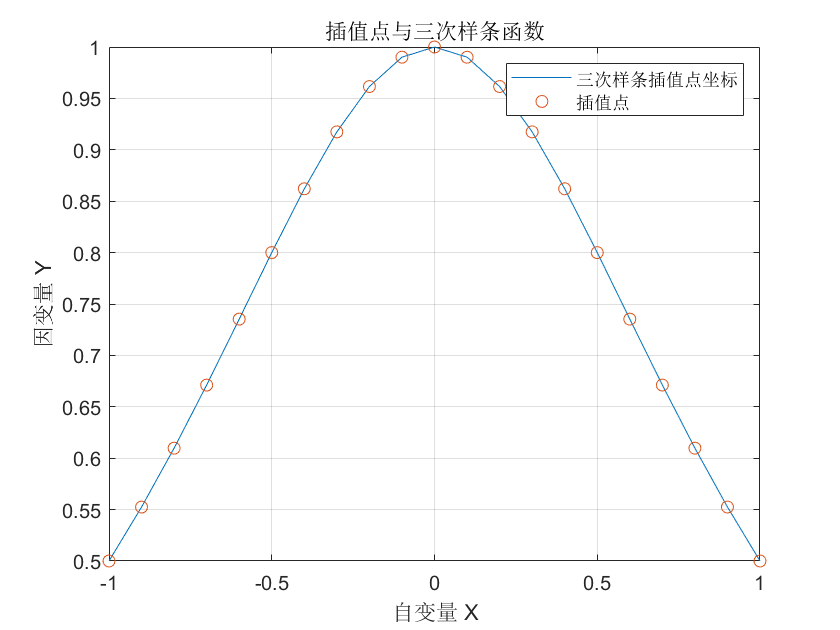
\includegraphics[width=0.5\textwidth,height=0.375\textwidth]{pictures/3sp1.png}
		\caption{第一类边界条件三次样条} \label{3sp1}
	\end{figure}


  \subsection{第二类边界条件}
  \subsubsection{代码展示}
  ~\\
  \lstset{language=matlab}
  \begin{lstlisting}
    clear;clc;
    x=-1:0.1:1;
    f=@(x)1./(1+x.^2);
    y=f(x);
    y0=0;          %  S''(x0)=f''(x0)=y0   
    yn=0;          %  S''(xn)=f''(xn)=yn
    x0=x;
    s=threesimple2(x,y,x0,y0,yn)
    plot(x0,s)        %绘制第二边界条件插值函数图像
    hold on
    grid on
    plot(x,y,'o')
    xlabel('自变量 X'), ylabel('因变量 Y')
    title('插值点与三次样条函数') 
    legend('三次样条插值点坐标','插值点')
    function [D,h,A,g,M]=three1(X,Y,y0,yn)
    %        自然边界条件的三次样条函数(第一种边界条件)
    %        此函数为M值求值函数
    %        D,h,A,g,M输出量分别为系数矩阵D,插值宽度h,差商表A,g值,M值 
             n=length(X); 
             A=zeros(n,n);A(:,1)=Y';D=zeros(n,n);g=zeros(n,1);
             for  j=2:n
                for i=j:n
                    A(i,j)=(A(i,j-1)- A(i-1,j-1))/(X(i)-X(i-j+1));
                end
             end
             
             for i=1:n-1
                 h(i)=X(i+1)-X(i);
             end
             for i=1:n
                 D(i,i)=2; 
                 D(1,2)=1;
                 D(n,n-1)=1;
                 if (i==1)
                     g(i,1)=6/h(i)*(A(2,2)-y0); 
                 elseif (i==n) 
                         g(i,1)=6/h(i-1)*(yn-A(i,2));
                 else 
                     g(i,1)=(6/(h(i-1)+h(i)))*(A(i+1,2)-A(i,2));
                 end
               
             end  
             for i=1:n-2
                 u(i)=h(i)/(h(i)+h(i+1));
                 n(i)=1-u(i);  
                 D(i+1,i+2)=n(i);
                 D(i+1,i)=u(i);             %改到这里
             end
             M=D\g;
             %M=[0;M;0];         
    end
    function s=threesimple1(X,Y,x,y0,yn)
    %        三次样条插值函数第一类型代码 
    %        s函数表示三次样条插值函数插值点对应的函数值
    %        根据三次样条参数函数求出的D,h,A,g,M
    %        x表示求解插值点函数点,X为已知插值点        
             [D,h,A,g,M]=three1(X,Y,y0,yn)
             n=length(X); m=length(x);    
             for t=1:m
                for i=1:n-1
                   if (x(t)<=X(i+1))&&(x(t)>=X(i))
                      p1=M(i,1)*(X(i+1)-x(t))^3/(6*h(i));
                      p2=M(i+1,1)*(x(t)-X(i))^3/(6*h(i));
                      p3=(A(i,1)-M(i,1)/6*(h(i))^2)*(X(i+1)-x(t))/h(i);
                      p4=(A(i+1,1)-M(i+1,1)/6*(h(i))^2)*(x(t)-X(i))/h(i);
                      s(t)=p1+p2+p3+p4; 
                      break;
                   else
                       s(t)=0; 
                   end
                end
             end
    end
    function [D,h,A,g,M]=three2(X,Y,y0,yn)
    %        第二边界条件的三次样条函数(包含自然边界条件)
    %        y0,yn表示的是S''(x0)=f''(x0)=y0,S''(xn)=f''(xn)=yn,自然边界即条件值为0 
    %        此函数为M值求值函数
    %        D,h,A,g,M输出量分别为系数矩阵D,插值宽度h,差商表A,g值,M值 
             n=length(X); 
             A=zeros(n,n);A(:,1)=Y';D=zeros(n-2,n-2);g=zeros(n-2,1);
             for  j=2:n
                for i=j:n
                    A(i,j)=(A(i,j-1)- A(i-1,j-1))/(X(i)-X(i-j+1));
                end
             end
             
             for i=1:n-1
                 h(i)=X(i+1)-X(i);
             end        
             for i=1:n-2
                 D(i,i)=2;
                 if (i==1)
                     g(i,1)=(6/(h(i+1)+h(i)))*(A(i+2,2)-A(i+1,2))-h(i)/(h(i)+h(i+1))*y0;
                 elseif (i==(n-2))
                     g(i,1)=(6/(h(i+1)+h(i)))*(A(i+2,2)-A(i+1,2))-(1-h(i)/(h(i)+h(i+1)))*yn;
                 else
                     g(i,1)=(6/(h(i+1)+h(i)))*(A(i+2,2)-A(i+1,2));
                 end             
             end
             for i=2:n-2
                 u(i)=h(i)/(h(i)+h(i+1));
                 n(i-1)=h(i)/(h(i-1)+h(i));
                 D(i-1,i)=n(i-1);
                 D(i,i-1)=u(i);             
             end
             M=D\g;
             M=[y0;M;yn];         
    end
    function s=threesimple2(X,Y,x,y0,yn)
    %        第二边界条件函数 
    %        s函数表示三次样条插值函数插值点对应的函数值
    %        根据三次样条参数函数求出的D,h,A,g,M
    %        x表示求解插值点函数点,X为已知插值点        
             [D,h,A,g,M]=three2(X,Y,y0,yn)
             n=length(X); m=length(x);    
             for t=1:m
                for i=1:n-1
                   if (x(t)<=X(i+1))&&(x(t)>=X(i))
                      p1=M(i,1)*(X(i+1)-x(t))^3/(6*h(i));
                      p2=M(i+1,1)*(x(t)-X(i))^3/(6*h(i));
                      p3=(A(i,1)-M(i,1)/6*(h(i))^2)*(X(i+1)-x(t))/h(i);
                      p4=(A(i+1,1)-M(i+1,1)/6*(h(i))^2)*(x(t)-X(i))/h(i);
                      s(t)=p1+p2+p3+p4; 
                      break;
                   else
                       s(t)=0; 
                   end
                end
             end
    end
  \end{lstlisting}
  \subsubsection{代码运行结果}
	\begin{figure}[!htbp]
		\centering
		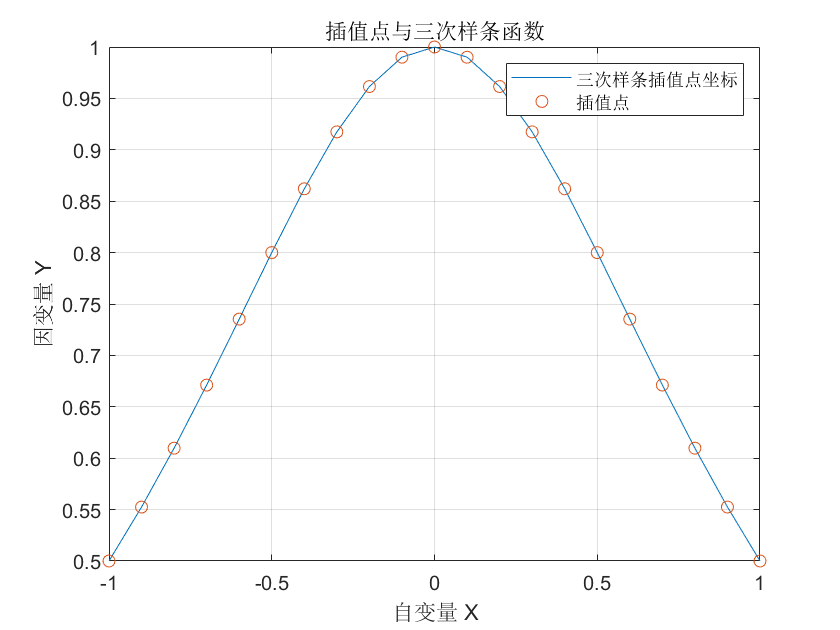
\includegraphics[width=0.5\textwidth,height=0.375\textwidth]{pictures/3sp2.png}
		\caption{第二类边界条件三次样条} \label{3sp2}
	\end{figure}

\section{题目四}
\subsubsection{代码展示}
~\\
\lstset{language=matlab}
\begin{lstlisting}
    clear;clc;
    x=[0.5;1.2;2.1;2.9;3.6;4.5;5.7];
    x_0=ones(length(x),1);
    t=0.5:0.01:5.7;
    x=[x_0,x];
    y=[2.81;3.24;3.80;4.30;4.73;5.29;6.03];
    s=x\y;
    T=s(1)+s(2)*t;
    disp("y轴截距a为"+s(1)+",回归系数b为"+s(2)+".")
    plot(x(:,2),y,'o')
    hold on
    plot(t,T,"k")
\end{lstlisting}


\subsubsection{代码运行结果}
y轴截距a为2.4991,回归系数b为0.61981.
\begin{figure}[!htbp]
    \centering
    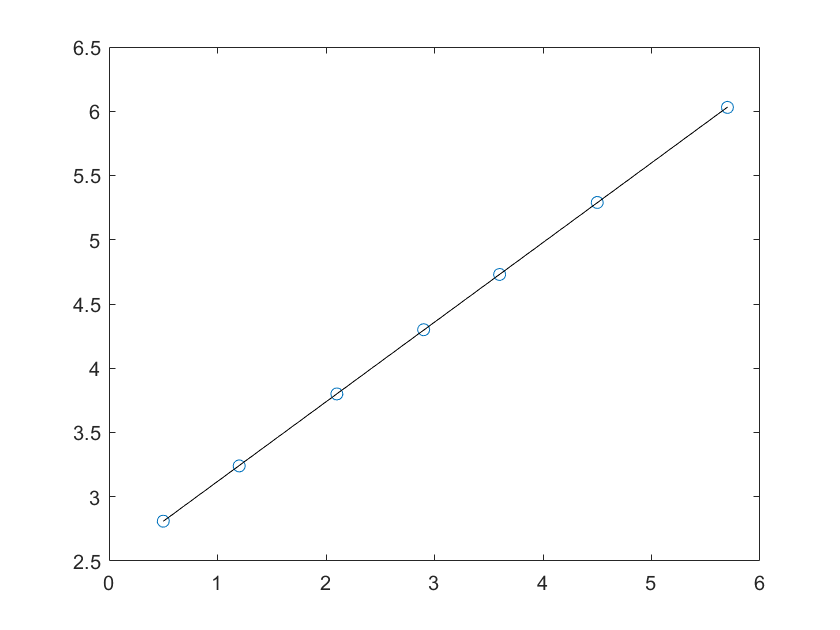
\includegraphics[width=0.5\textwidth,height=0.375\textwidth]{pictures/linearfit.png}
    \caption{数据点及其拟合的直线} \label{linearfit}
\end{figure}
\newline
%%%以下为插入图片模板
%\quad \newline
%	\begin{figure}[!htbp]
%		\centering
%		\includegraphics[width=0.5\textwidth,height=0.375\textwidth]{pictures/minscale.png}
%		\caption{最小风向} \label{minsacle}
%	\end{figure}

%%%以下为插入图片模板
%\quad \newline
%	\begin{figure}[!htbp]
%		\centering
%		\includegraphics[width=0.5\textwidth,height=0.375\textwidth]{pictures/minscale.png}
%		\caption{最小风向} \label{minsacle}
%	\end{figure}

%    \begin{algorithm}
%		\caption{Title of the Algorithm}
%     	\begin{algorithmic}[1]
%			\REQUIRE some words.  % this command shows "Input"
%			\ENSURE ~\\           % this command shows "Initialized"
%			some text goes here ... \\
%			\WHILE {\emph{not converged}}
%			\STATE ... \\  % line number at left side
%			\ENDWHILE
%			\RETURN this is the lat part.  % this command shows "Output"
%		\end{algorithmic}
%	\end{algorithm}

\end{document}